\chapter{Motivation}

Als Fake News werden Falschmeldungen bezeichnet, die mit manipulativer Absicht viral verbreitet werden. In dem 
"Whitepaper"\cite{facebook}, was Facebook am 27.04.2017 veröffentlichte, werden vier verschiedene Motive und  
Methoden von Falschnachrichten beschrieben. Zum einen mit der Absicht anhand von Fake News politische Stimmungen 
zu steuern, zum anderen mithilfe von Fehlinformationen bestimmt Gefühle zu erzeugen oder Aufmerksamkeit zu erzielen. 
Ein weitere Methode kann das manipulieren von politischen Diskussionen mithilfe von koordinierten Aktivitäten sein und 
zu letzt die bloße Desinformation.

Die Motive und Methoden werden immer komplexer und aufgrund der hohen Lukrativität\cite{Cynk} wird es immer schwieriger 
ohne große Eigenrecherche zu erkennen, ob die Nachricht der Wahrheit entspricht oder eine Falschmeldung ist.
Da eine Verbreitung in sozialen Netzwerken deutlich einfacher ist und diese Platformen zunehmend als einzige
Informationsquelle genutzt werden, wächst die Gefahr die von Fake News ausgeht.
Auch die Verbreitung von Nachrichten ist in sozialen Netzwerken deutlich leichter und Falschmeldungen sind schwer 
zu revidieren. 
Daher besteht ein großes Interesse darin, schnell zu wissen, ob Nachrichten der Wahrheit entsprechen oder nicht, um 
eine Verbreitung früh zu unterbinden. 

Eine Überprüfung des Inhalts würde zu viel Zeit in Anspruch nehmen. Eine schnellere Möglichkeit wäre eine Analyse 
des Textes mithilfe von Natural Language Processing und Neuronal Networks.
Dabei werden sowohl Kontext als auch Schreibstil des Textes analysiert und dann anhand dieser Information eine 
Likelihood bestimmt zu der ein Text "Fake" oder "Real" ist.
Diese Methode kann eine Überprüfung des Inhalts nicht ersetzen, 
jedoch könnte es bei einer ausreichenden Genauigkeit zu einem vorläufigen Sperren der Nachricht führen, was die 
unaufhaltsame Verbreitung dieser Falschmeldung verhindern würde.

Eine schon vorhandene Möglichkeit Fake News zu detektieren ist der "B.S. Detector" von Daniel Sieradski\cite{BS}.
Diese Browser Erweiterung überprüft alle verlinkten Webseiten auf verdächtige Quellen, indem es die Domains 
mit einer manuell gepflegten Liste von unzuverlässigen Quellen vergleicht. Dieses Tool hat das Problem, dass 
die Liste manuell geführt werden muss und es durch Vermeiden der fragwürdigen Domains möglich ist, den Filter zu 
umgehen. 

\chapter{Struktur und Verarbeitung des Datensatzes}
\label{sec:struct}

Der Datensatz besteht zu $44\%$ aus Nachrichten die vom B.S. Detektor detektiert wurden und zu $56\%$ aus gesammelten 
Nachrichten von vertrauenswürdigen Nachrichtendiensten, wie die Washington Post oder die New York Times. Die Nachrichten 
sind hauptsächlich auf Englisch und die Falschnachrichten sind vom 25.Oktober.2016 bis 25.November.2016 gesammelt worden. Für den Zeitraum 
der Real News ist Oktober bis November 2016 angegeben. 
Der Fake News Datensatz ist auf Kaggle.com zu finden\cite{fake_data} und die Real News werden in einem Kernel hinzugefügt\cite{real_data}.
Nach Aussortieren der nicht englischsprachigen Texte mithilfe der \textsc{langdetect}-Bibliothek\cite{langdetect}, welche die
Language Detection Bibliothek von Google\cite{google_langdetect} nutzt, hat der gesamte Datensatz eine Größe von 
$\num{27903}$.

Aufgrund des gegebenen Datensatzes kann die Fragestellung dieser Arbeit nur eingeschränkt formuliert werden.
Mithilfe dieses Datensatzes kann keine allgemeine Fake News Erkennung trainiert werden, da hier nicht der Inhalt 
ausschlaggeben für die Klassifizierung der Trainingsdaten ist, sondern der B.S. Detektor und somit die Quellen des 
Artikels. 
Zudem gibt es in dem Real News Datensatz nur $10$ verschiedene Herausgeber.
Daher hat der Datensatz eine große Verzerrung und es kann nur darauf trainiert werden, ob Texte vom B.S. Detektor 
als fragwürdig klassifiziert werden würden oder ob sie von einem der $10$ als glaubwürdig erachteten Herausgebern stammt.

Zunächst wird der Datensatz mithilfe der \textsc{nltk}-Bibliothek\cite{nltk} durch Lemmatisierung verarbeitet, um 
alle Wörter auf ihre Stammform zurückzuführen (siehe \ref{sec:NLP}). 
Anschließend werden die Worthäufigkeiten in jedem Text mithilfe der \textsc{scikit-learn}-Bibliothek\cite{scikit-learn} 
gezählt. 
Somit ergibt sich das Bag-of-words Modell als Repräsentation des Textes.
Auf eine Aussortieren der Stoppwörter wird verzichtet, da diese zwar nicht relevant für den Inhalt der Nachricht sind,
jedoch Teil des Schreibstils sind und somit relevant für eine Trennung sein können.

\begin{comment}
    \begin{figure}[t!]
    \centering
    \begin{subfigure}[t]{0.45\textwidth}
        \centering
        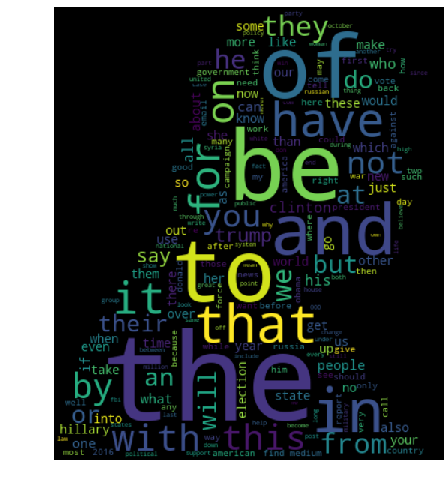
\includegraphics[width=\textwidth]{pictures/fake_wordcloud.pdf}
        \caption{Fake News}
    \end{subfigure}
    \begin{subfigure}[t]{0.54\textwidth}
        \centering
        \raisebox{1.5cm}[0pt]{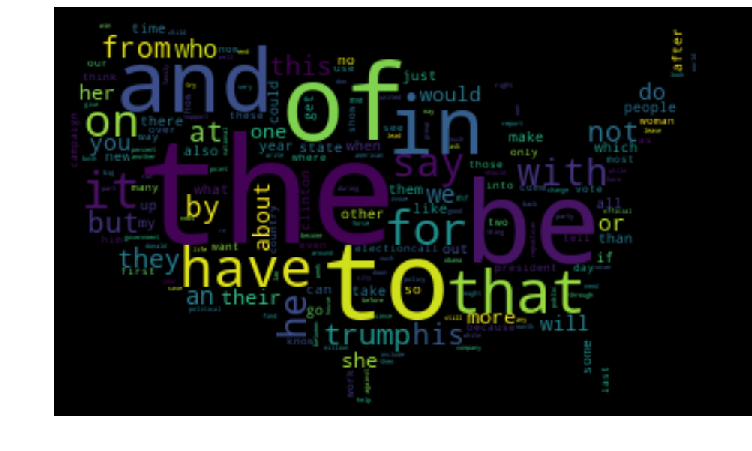
\includegraphics[width=\textwidth]{pictures/real_wordcloud.pdf}}
        \caption{Real News}
    \end{subfigure}
    \caption{Mit \textsc{wordcloud} \cite{wordcloud} erstellte Darstellung der Worthäufigkeiten für Real und Fake News.}
    \label{fig:wordcloud}
    \end{figure}
\end{comment}



\chapter{Lösungsansatz}

\begin{figure}
    \centering
    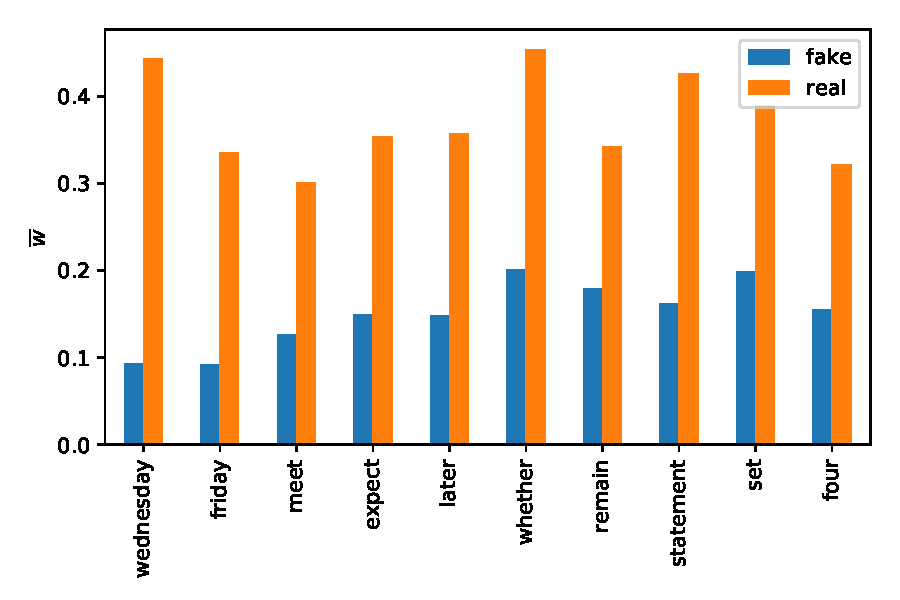
\includegraphics[width=0.8\textwidth]{pictures/data_visualisation.pdf}
    \caption{Darstellung der relativen Worthäufigkeit der $10$ Wörter, mit maximaler Differenz der Mittelwerte.
            Eine Unterschied ist klar zu erkennen, wobei ein Teil dadurch erklärt ist, dass die Texte der Real 
            News im Mittel $\approx 1590$ Zeichen länger sind.}
    \label{fig:word_plot}
\end{figure}
Um zu veranschaulichen, ob ein Unterschied der Worthäufigkeiten im Fake- und Real-News Datensatz besteht, werden in \ref{fig:word_plot}
die $10$ Wörter, die am besten zur Trennung geeignet sind, dargestellt. 
Als Kriterium wird 
\begin{equation}
    \frac{(\overline{w_{real}}-\overline{w_{fake}})^2}{s_{real}^2+s_{fake}^2}
\end{equation}
verwendet, welches von der ein dimensionalen linearen Fisher Diskriminanzanalyse inspiriert ist. 
Dabei ist $\overline{w_k}$ das arithmetische Mittel und $s_{k}^{2}=\sum_{i=1}^{N_{k}}\left(w_{k i}-\overline{w}_{k}\right)^{2}$ 
die Summe der quadrierten Abweichungen.
Wörter mit großen Distanzen zwischen den Mittelwerten relativ zu der Streuung können gut zur Trennung genutzt werden.
In \ref{fig:word_plot} ist zu erkennen, dass Real und Fake News durchaus anhand der Worthäufigkeit zu unterscheiden sind. 
Gründe können zum einen Unterschiede in der Ausdrucksweise sein und zum anderen unterschiedliche Themenbereiche. Da die 
Wörter in \ref{fig:word_plot} keine themenspezifischen Worte sind, deutet es daraufhin, dass eher eine unterschiedliche 
Ausdrucksweise ausschlaggeben ist. 
Zum Beispiel scheinen genaue Wochentage in Real News häufiger verwendet zu werden. 
Das kann zum Teil daher bekommen, dass bei Fakten ein genauer Zeitpunkt erwähnt werden kann und bei Falschnachrichten, die 
nur auf eine emotionale Reaktion zielen, ist der genaue Zeitpunkt des Ereignisses nicht existent und auch nicht relevant.
Zu beachten ist, dass Real News im Mittel $\num{1590}$ Zeichen länger sind als Fake News und somit die relative Häufigkeit 
generell bei Real News höher ist als bei Fake News. 
Dies ist jedoch auch ein Attribut was aus dem BoW Modell generiert und genutzt werden kann.
Desweiteren scheinen Stoppwörter, wie "whether", relevant zu sein, weshalb sie mit in die Analyse genommen werden.

Um zu genneralisieren, werden nur die $500$ im Trainingsdatensatz am häufigsten verwendeten Wörter als Attribute 
für die Input-Lage des Deep feedforward Neural Networks verwendet. 
Jedoch wird lieber eine L1-Regularizierung in der ersten hidden Layer verwendet, um ein overfitting zu verhindern, 
anstatt die Anzahl der Wörter zu verringern, da, wie in \ref{fig:word_plot} zusehen, häufig verwendete Wörter nicht 
zwangsweise gut zur Trennung geeignet sein müssen.

\begin{figure}
    \centering
    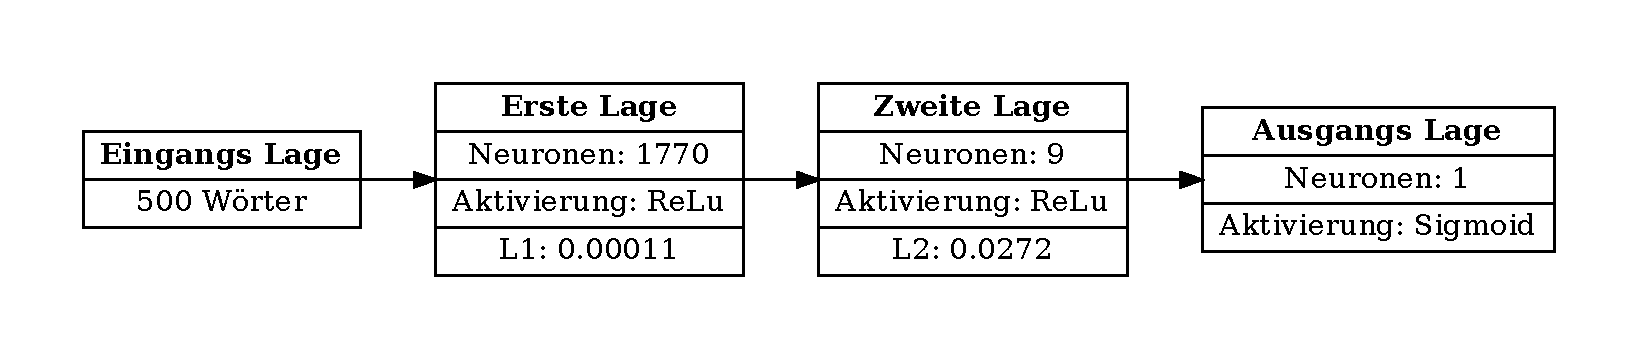
\includegraphics[width=\textwidth]{pictures/modell_scheme.pdf}
    \caption{Graphische Darstellung des optimierten Modells. Es wurden Tiefe, Breite und Regularizierung mithilfe 
            des Tree of Parzen Estimator Algorithmus (siehe \ref{sec:TPE}) optimiert.}
    \label{fig:NN_structure}
\end{figure}

Das mit Keras\cite{keras} aufgebaute Netz wird mithilfe der \textsc{hyperas}-Bibliothek\cite{hyperas} optimiert und 
es ergibt sich ein optimaler Classifier, wie er in \ref{fig:NN_structure} dargestellt ist.
Als Verlustfunktion stellt sich die binäre Kreuzentropie als optimal heraus und als Optimierer der Adagrad Algorithmus.
Bei dem Adagrad Optimierungs Algorithmus für die Optimierung der Gewichte werden die Standard Einstellungen verwendet, 
da eine Optimierung der Lernrate und der Zerfallsrate nur zu einem unbeständigen Training geführt hat.


\chapter{Ergebnisse}

\begin{figure}[t!]
    \centering
    \begin{subfigure}[t]{0.49\textwidth}
        \centering
        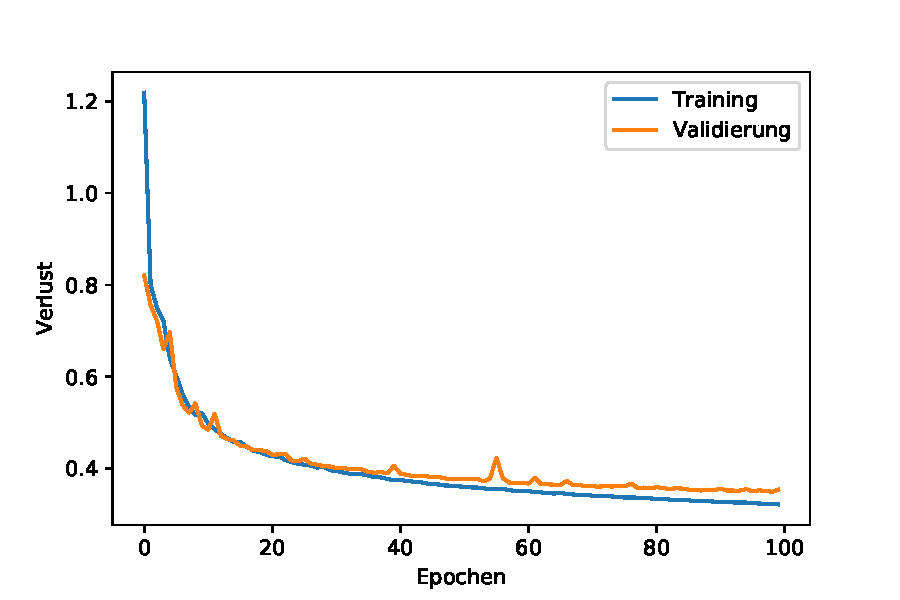
\includegraphics[width=\textwidth]{pictures/history_bow_best.pdf}
        \caption{Abbildung des Trainingsfehler und des Validierungsfehlers im Laufe des Trainings.}
        \label{fig:history}
    \end{subfigure}
    \begin{subfigure}[t]{0.49\textwidth}
        \centering
        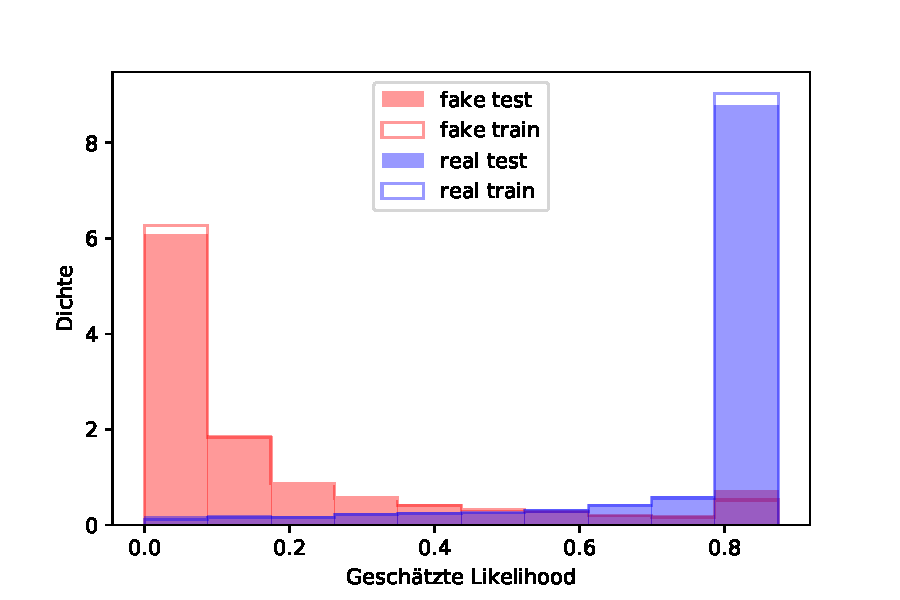
\includegraphics[width=\textwidth]{pictures/prob_bow_best_nn.pdf}
        \caption{Darstellung der Vorhersage bei Trainings und Testdatensatzes.}
        \label{fig:probs}
    \end{subfigure}
    \caption{Analyse des Modells auf ein mögliches Übertraining.}
\end{figure}
Das Modell wird über $100$ Epochen trainiert und über die Epochen der Trainingsfehler und der Validierungsfehler 
berechnet und in \ref{fig:history} dargestellt. 
Da eine Batch Size von $64$ genutzt wird, ist ein langsames Training zu beobachten, jedoch besitzt die Berechnung 
des Gradienten weniger Fluktuationen und es ist wahrscheinlicher das globale Minimum zu finden. 
Ab $\approx 40$ Epochen ist das Modell nahezu ausgelernt und der Validierungsfehler bleibt nahezu konstant und 
nur der Trainingsfehler sinkt. 
Ab diesem Punkt beginnt das Modell leicht überzutrainieren, jedoch besteht kein starkes Übertraining, was auch in 
\ref{fig:probs} zusehen ist.
Die vorhergesagten Likelihoods sind bei Trainings- und Validierungsdatensatz nahezu gleich verteilt.
Die Verteilungen sind mit einem Schnitt bei $0.5$ gut zu trennen, was auf eine Genauigkeit von $0.86$ für die 
Fake News Klassifizierung und eine Genauigkeit von $0.90$ für die Real News Klassifizierung führt.
Jedoch führt die Breite der Fake News Verteilung auf eine erhöhte Kreuzentropie von $0.32$.

\begin{figure}[t!]
    \centering
    \begin{subfigure}[t]{0.49\textwidth}
        \centering
        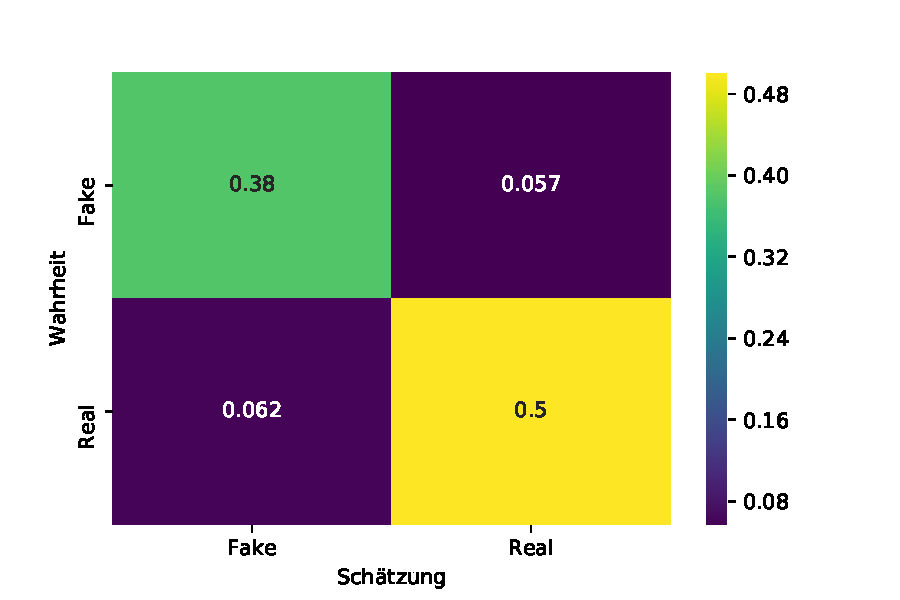
\includegraphics[width=\textwidth]{pictures/cnfsn_mtx_bow_best_nn.pdf}
        \caption{Confusion Matrix}
        \label{fig:CM}
    \end{subfigure}
    \begin{subfigure}[t]{0.49\textwidth}
        \centering
        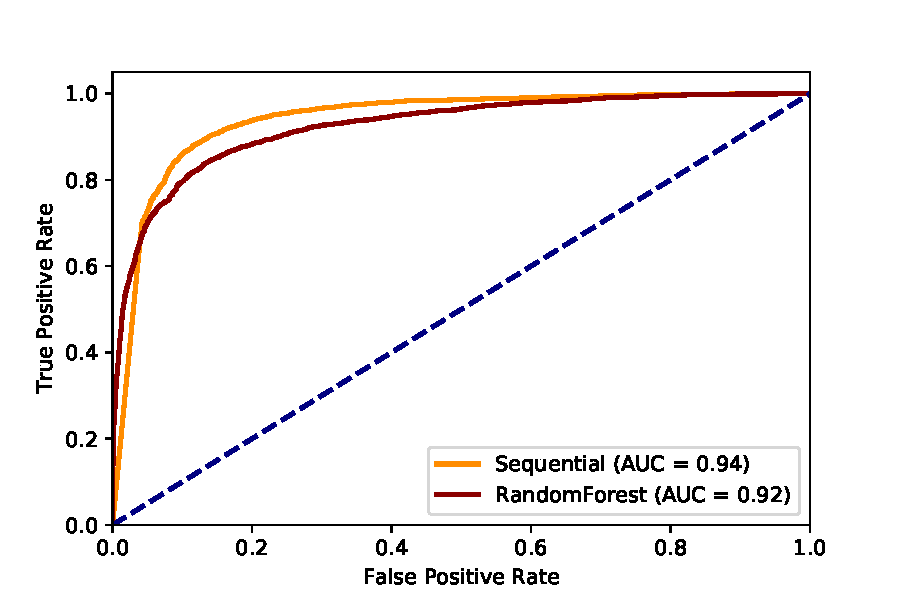
\includegraphics[width=\textwidth]{pictures/roc_comparison.pdf}
        \caption{Receiver Operating Characteristic(ROC)}
        \label{fig:ROC}
    \end{subfigure}
    \caption{Darstellung der Performanz des trainierten Classifiers auf dem unabhängigen Testdatensatz. In \ref{fig:ROC}
            ist zusätzlich die Performanz des Random Forests abgebildet, welcher als Vergleichsmethode dienen soll.}
\end{figure}
In \ref{fig:CM} ist die Vorhersage des Neuronalen Netzes in einer Confusion Matrix dargestellt. 
Da die Nebendiagonalen etwas $12\%$ der Daten beinhalten und beide Diagonalelemente(True Positive and True Negative) 
relativ zum Datenanteil der Wahrheiten gleichermaßen ausgeprägt sind, kann von einem erfolgreichen Training gesprochen 
werden.
Auch die Receiver Operating Characteristic(ROC) mit einem Area under Curve(AUC) Wert von $0.94$ spricht dafür, dass 
der Classifier eine Struktur in den Daten erkannt hat.
Auch die ROC Kurve zeigt die Schwäche des Modells bei der Erkennung von Fake News, wie auch in \ref{fig:probs} zusehen.

\begin{figure}
    \centering
    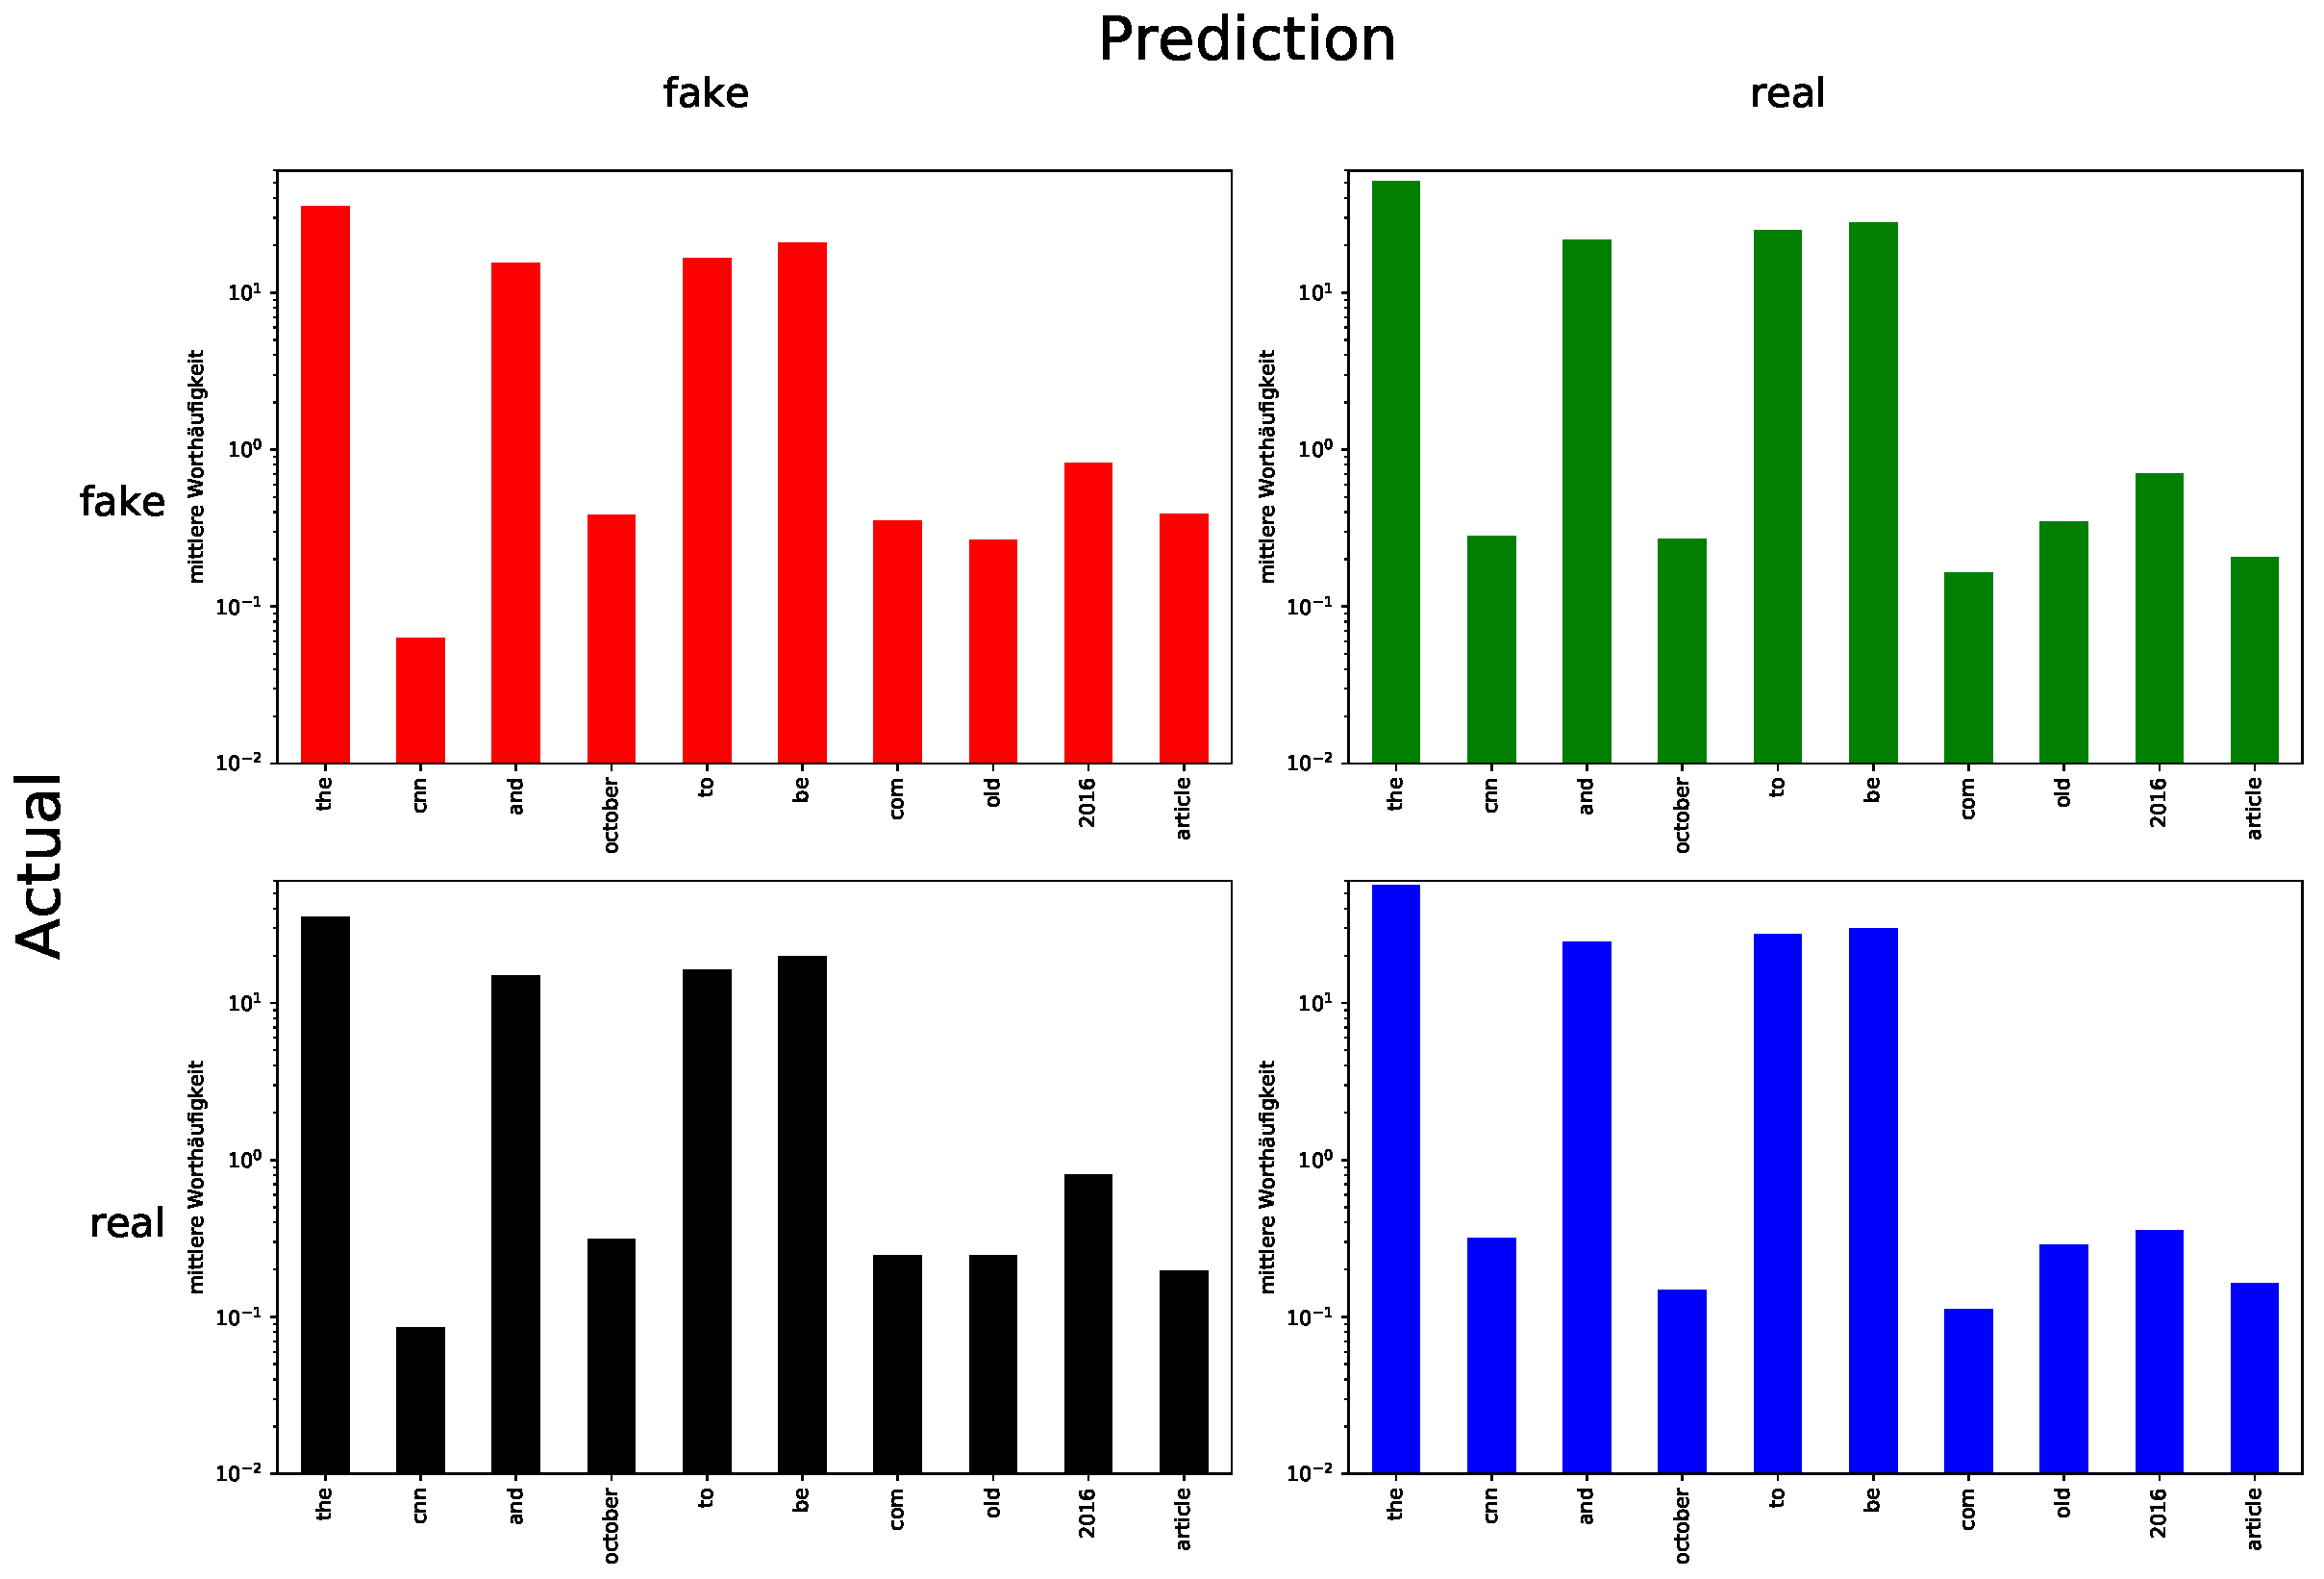
\includegraphics[width=\textwidth]{pictures/cnfn_hist.pdf}
    \caption{Untersuchung der Fehlklassifizierungen mithilfe der Worthäufigkeiten von Worten denen vom 
            Modell eine hohe Wichtigkeit beigemessen wird.}
    \label{fig:CM_i}
\end{figure}
Um die Trennung besser zu verstehen, wird die erste Lage des Neuronalen Netzes genauer untersucht.
Dabei wird
\begin{equation}
    g_i = \sum_{j=1}^{N_2}|w_{ij}|
\end{equation}
als Wichtigkeit des Wortes $w_i$ interpretiert. Dabei ist $w_{ij}$ das Gewicht von Attribut $i$ zum Neuron $j$ der 
ersten versteckten Lage und $N_j=1770$ die Breite dieser Lage.
Die mittlere Häufigkeit der $10$ wichtigsten Worte werden in \ref{fig:CM_i} für die richtig und falsch klassifizierten 
Texte dargestellt.
Deutlich zu erkennen ist, dass die Histogramme wie erwartet bei der gleichen Schätzung eine fast gleiche Struktur besitzen.
Außerdem spielen Stoppwörter wie "the", "to", "and" und "be" eine zentrale Rolle in der Trennung.
Die Stoppwörter sind klar mit der Textlänge korreliert und da Texte der Real News im Mittel $\num{1590}$ Zeichen 
länger sind, klassifiziert das Modell, wie in \ref{fig:CM_i} zu sehen, Texte mit einer höheren Worthäufigkeit bei Stoppwörtern 
als Real News.
Das Wort "cnn" wird von dem Neuronalen Netz auch als Indiz für einen Real News Text gesehen.
Dies ist vielleicht damit zu begründen, dass wahre und seriöse Nachrichten sich auf Quellen, wie CNN beziehen und 
Falschmeldungen keine seriöse Quelle besitzen.
Das Wort "com" ist ein Indiz auf Internetseiten und kommt in Texten die als Fake News klassifiziert werden häufiger 
vor.
Zum einen kann das daran liegen, dass Fake News häufiger Internetquellen haben, jedoch liegt es auch daran das die 
genutzen Fake News Texte einen freiere blogähnliche Schreibstruktur aufweisen. 
Im Gegensatz zu den seriösen und strikten Bericht Strukur der Nachrichten aus seriösen Nachrichtendiensten wie die 
Washington Post.
In \ref{fig:CM_i} ist jedoch auch zu erkennen, dass die $10$ Wörter in einer der beiden Kategorien im Schnitt mindestens in 
jedem fünften Text vorkommen. 
Dies deutet auf eine Generalisierung hin, jedoch sind Wörter wie "2016" klar Zeitbezogen und Texte aus einem anderen 
Zeitraum werden für das trainierte Modell deutlich schwerer zu klassifizieren sein. 

Um Beurteilen zu können, ob das aufwendige Training eines tiefen Neuronalen Netzes notwendig ist oder ob eine einfachere
Methode des Maschinellen Lernens ähnliche Ergebnisse liefert, wird in \ref{fig:ROC} auch die Performanz eines 
Random Forests dargestellt. 
Der Random Forest nutzt genau wie das Neuronale Netz die Worthäufigkeiten des Bag of Words Modells, jedoch 
werden einfache Schnitte in den Merkmalen verwendet um die Daten zu klassifizieren.
Der Random Forest besitzt $100$ Entscheidungsbäume mit einer maximalen Tiefe von $10$ und als Trennkriterium wird die 
Informationsentropie verwendet.
\ref{fig:ROC} zeigt, dass das Neuronale Netz mit einem AUC Wert von $0.94$ besser klassifiziert als der Random Forest
mit einem AUC Wert von $0.92$.
Jedoch erkennt der Random Forest die Fake News mit einer Genauigkeit von $0.87$ wie das Neuronale Netz und ist, wie 
in der ROC Kurve zu sehen für sehr niedrige Schnitte sogar besser.
Jedoch ist die Genauigkeit bei der Erkennung der Real News mit $0.81$ deutlich schlechter. 
Da in die Hyperparameter Optimierung des Random Forests nicht so viel Zeit wie in die Optimierung des Neuronalen 
Netzes investiert wurde, kann nicht zwingend von einer Überlegenheit des Neuronalen Netzes gesprochen werden.

\chapter{Zusammenfassung}

Abschließend ist festzustellen, dass eine Fake News Erkennung anhand von Worthäufigkeiten in den Nachrichten möglich 
ist.
Eine durchschnlittliche Genauigkeit von $0.88$ lässt darauf schließen, dass Unterschiede in Fake und Real News erfasst
werden können, jedoch zeigt \ref{fig:probs} und \ref{fig:CM_i} deutlich, dass einige Falschnachrichten große 
Ähnlichkeiten mit wahren Nachrichten haben und somit schwer zu klassifizieren sind.

Jedoch müssen die schon in \ref{sec:struct} erwähnten Einschränkungen in der Definition der Fragestellung noch einmal 
hervorgehoben werden.
Die Etikettierung des Datensatzes mithilfe des B.S. Detektors ist keine wahre Fake News Erkennung, da nicht der 
Wahrheitsgehalt der Texte überprüft wird, sondern nur eine Schwarze Liste von fragwürdigen URLs zu Klassifizierung 
benutzt wird.
Daher sind die in diesem Datensatz als Fake News klassifizierten Nachrichten nicht zwangsläufig Falschnachrichten. 
Die Klassifizierung, die in dieser Arbeit vorgenommen wird, ist strenggenommen ein Filter, der Texte von 
vertrauenswürdigen Zeitungen und Artikel von Webseiten mit Verbindungen zu URLs auf der Schwarzen Liste trennt.
Dies begünstigt die Trennung, da der Schreibstil und die Struktur der Texte aufgrund der unterschiedlichen Herkunft 
durchaus abweichen können. 
Die Frage, ob der Unterschied in Stil und Struktur eine Verzerrung im Datensatz bewirkt oder ob dies ein 
legitimes Merkmal darstellt, ist schwer zu beantworten.

Eine klare Verzerrung die in diesem Datensatz besteht, ist jedoch die Tatsache, dass die Daten in einem festen 
Zeitraum aufgenommen wurden.
Da jedoch die Thematik der Nachrichten in einem anderen Zeitraum vollkommen unterschiedlich sein kann, wird das 
Modell Nachrichten aus anderen Zeiträumen nicht so gut trennen können.
\ref{fig:CM_i} zeigt jedoch, das durchaus von einer Generalisierung gesprochen werden kann, jedoch besitzt die 
Zahl "2016" ein deutliches Gewicht bei der Trennung.
Die Wichtigkeit des Wortes leitet sich jedoch aus dem begrenzten Zeitraum des Datensatzes her.

Da die Performanz des Random Forests nahe an der des Neuronalen Netzes liegt und der Bau des Entscheidungsbaumes 
nur eine Zeitkomplexität von $\Omega(n \log^2 (n))$\cite[96]{understanding_RF} besitzt, ist die Notwendigkeit des 
Trainings eines tiefen Netzes nicht zwangsläufig gegeben.
Jedoch besitzt das Neuronale Netz mehr Potential, bei einem größeren Datensatz und einer größerern Rechenkapazität.
Auch andere NLP Methoden wie "word2vec" oder der BERT Encoder\cite{bert} sind vielversprechende Methoden, die jedoch 
größere Neuronale Netze benötigen. 
Eine einfache Analyser der Nachrichten Überschriften mithilfe des Bert Encoders und eines feedforward Neuronalen 
Netzes besitzt eine Genauigkeit von $0.77$. 
Die Verarbeitung von ganzen Texten ist jedoch zu rechenaufwendig für dieses Projekt und konnte nicht weiter 
verfolgt werden.
Eine andere vielversprechende Methode sind die rückkoppelnden Neuronalen Netze.
Beide Methoden besitzen die Möglichkeit den Kontext des Textes und nicht allein die Worthäufigkeiten bei der 
Trennung mit zu berücksichtigen, jedoch ist eine Interpretation der Trennung deutlich schwieriger bis nicht möglich.




\chapter{code}
github Link

\appendix
\chapter{Natural Language Processing}
\label{sec:NLP}

\chapter{Bayesian Optimization}
\label{sec:TPE}
